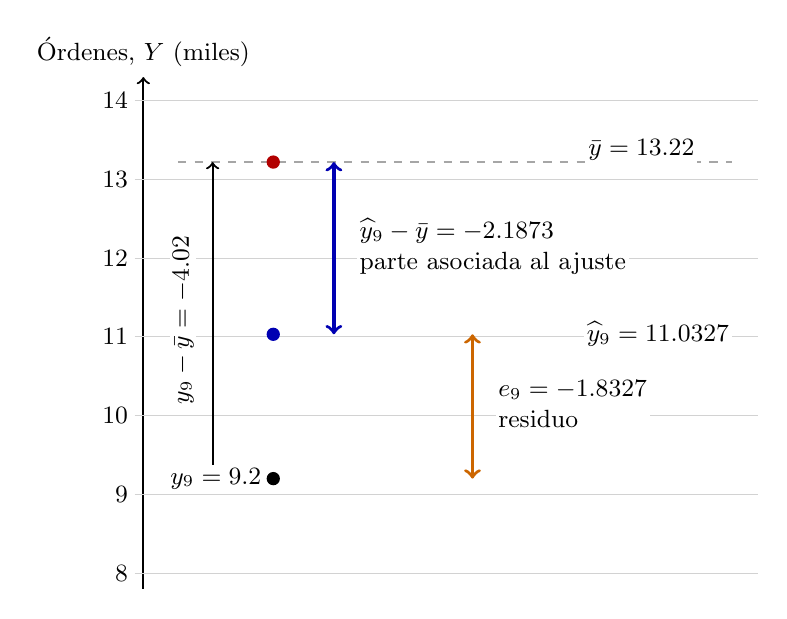
\begin{tikzpicture}[x=2.2cm,y=1cm,font=\small]
    \draw[->,thick] (-0.75,7.8) -- (-0.75,14.3) node[above] {Órdenes, $Y$ (miles)};
    \foreach \yy in {8,9,10,11,12,13,14} {
        \draw[gray!35] (-0.8,\yy) -- (2.8,\yy);
        \node[left=2pt] at (-0.75,\yy) {\yy};
    }
    \draw[gray!70,dashed,thick] (-0.55,13.22) -- (2.65,13.22);
    \node[anchor=west,fill=white,inner sep=1pt] at (1.8,13.38) {$\bar y=13.22$};
    \draw[black,<->,thick] (-0.35,9.2) -- (-0.35,13.22);
    \node[rotate=90,fill=white,inner sep=1pt] at (-0.52,11.21) {$y_9-\bar y=-4.02$};
    \draw[blue!70!black,<->,very thick] (0.35,11.0327) -- (0.35,13.22);
    \node[anchor=west,align=left,fill=white,inner sep=1pt] at (0.48,12.15) {$\widehat y_9-\bar y=-2.1873$\\parte asociada al ajuste};
    \draw[orange!80!black,<->,very thick] (1.15,9.2) -- (1.15,11.0327);
    \node[anchor=west,align=left,fill=white,inner sep=1pt] at (1.28,10.15) {$e_9=-1.8327$\\residuo};
    \fill[black] (0,9.2) circle (2.4pt);
    \fill[blue!70!black] (0,11.0327) circle (2.4pt);
    \fill[red!70!black] (0,13.22) circle (2.4pt);
    \node[anchor=east,fill=white,inner sep=1pt] at (-0.05,9.2) {$y_9=9.2$};
    \node[anchor=east,fill=white,inner sep=1pt] at (2.65,11.0327) {$\widehat y_9=11.0327$};
\end{tikzpicture}